\documentclass[aps,twocolumn,secnumarabic,nobalancelastpage,amsmath,amssymb,
nofootinbib,floatfix]{revtex4}
\usepackage{graphics}      % especificaciones gráficas estándar
\usepackage{graphicx}      % especificaciones alternativas para lso gráficos
\usepackage{longtable}     % ayuda con las opciones de tablas grandes
\usepackage{url}           % para referencias en línea
\usepackage{bm}            % paquete especial 'bold-math'
\usepackage[utf8]{inputenc}
\usepackage[english]{babel}


\usepackage{natbib} 


\begin{document}
\title			{Computational study of carbon nanoscrolls as cathodes in alluminum batteries}
\author         {Tomás Rojas Solorzano}
\affiliation    {Sede de Occidente, Universidad de Costa Rica}
\author         {Dale Igram}
\affiliation    {University of Michigan}
\author         {Leandro Ruiz Hernández}
\author         {Hernán Barquero}
\email          {leandro.ruiz@ucr.ac.cr}
\homepage       {http://www.fisica.ucr.ac.cr}
\affiliation    {Escuela de Física, Universidad de Costa Rica}
\date{\today}


\begin{abstract}
Aluminum-ion batteries (AIBs) present a sustainable and cost-effective alternative to lithium-ion technology, offering high volumetric capacity and reduced environmental impact. In this work, we investigate the performance of Carbon Nanoscrolls (CNS) as a novel cathode material for AIBs using Density Functional Theory (DFT) and Molecular Dynamics (MD) simulations. We constructed an Archimedean spiral CNS model and analyzed its interaction with the AlCl$_3$/[Emim]Cl ionic liquid electrolyte. Our results demonstrate the stable adsorption of AlCl$_4^-$ anions within the nanoscroll galleries, with a preference for tetrahedral configurations. Projected Density of States (PDOS) analysis reveals significant hybridization between the intercalant and the carbon host near the Fermi level, facilitating charge transfer. Furthermore, MD simulations over 3.5 ps indicate the rapid formation of a stable Solid Electrolyte Interphase (SEI), characterized by a strong ordering of ionic species at the interface as confirmed by Radial Distribution Functions (RDFs). These findings suggest that CNSs are promising candidates for high-performance AIB cathodes.
\end{abstract}

\maketitle


\section{Introduction}

Lithium batteries have been widely used over the years\cite{leisegang2019aluminum}, becoming the most common type among chemical energy storage systems, particularly in the field of electric vehicles\cite{zeng2019commercialization}. However, this technological advancement has raised various concerns related to the ethics and sustainability of lithium mining, as well as the management and disposal of these batteries at the end of their life cycle\cite{mrozik2021environmental}. The recycling process is rigorous due to hazards to workers, which can be electrical, explosive, or chemical\cite{diekmann2017potential}. Furthermore, environmental risks persist if they are improperly disposed of; according to Sommervile \cite{sommerville2020review}, only 5\% of lithium batteries were properly disposed of in 2019 in the European Union, and there are currently no international standards for their disposal\cite{mrozik2021environmental}.\\
Our paper aims to analyze the performance of aluminum batteries as an alternative to traditional lithium-based ones, through the analysis of carbon nanoscrolls as cathode materials\cite{Jung2016Flexible}. Given the behavior of aluminum in the presence of ionic liquids, the cathode largely determines the overall performance of the battery\cite{mishra2022design}.\\
Aluminum is the most abundant metal in the Earth’s crust, and its extraction does not pose significant environmental risks\cite{leisegang2019aluminum}. This element stands out for its high volumetric capacity, defined as the amount of energy a battery can store per unit of volume. These findings are consistent with those reported by Yang, who highlights the low extraction cost of aluminum and its superior volumetric capacity compared to other metals.\\
The cathode material also plays a significant role in the simulation, since carbon based cathodes offer a good alternative to the more traditional metal oxide cathodes. One of the biggest advantages that carbon cathodes is that they are cheaper and easier to produce using various synthesis methods \cite{Wang2018facile,Zhang2018Low}, according to Zhou, the carbon based cathodes offer an excellent stability and high electronic conductivity in lithium batteries.\cite{zhou2022carbon},\cite{gupta2024aluminum}. \\
Despite all of this one of the main challenges of the comercialization of Alluminum based batteries is the stability of the cathode with the interaction of AlCl$_4$ which carbon based cathodes have shown promissing results.\cite{ambroz2017trends}
Agiorgious emphasizes that the selection of the ionic liquid is a critical factor, because aluminum generally requires a corrosive electrolyte to prevent oxidation\cite{agiorgousis2017role}. A combination of AlCl$_3$ and EMImCl (1-ethyl-3-methyl-imidazolium chloride) is proposed as a suitable electrolyte system for this type of battery. This study employs a liquid mixture of EMIm-Cl and AlCl$_3$.\\



This paper seeks to build upon the results obtained by Liu, whose research demonstrated a high energy capacity in cathodes based on carbon nanoscrolls, along with stable performance across a wide temperature range with a good reversible specific capacity even after 55000 cycles. It also offers a rapid electron transmission and a significant anion storage capability and an ultrafast charge and slow discharge rate. These carbon structures allow the cathode to expand and change while maintaining stability, although structural defects such as Stone-Wales defects can significantly influence these properties \cite{Jha2018Role,Tiwari2023Stone,Wang2013Catalytically}. It is particularly relevant to analyze the possible configurations that AlCl$_4$molecules can adopt within the nanoscroll, as there is still no consensus regarding which of the three stable configurations is most likely or energetically favorable \cite{liu2018carbon,Chen2022Formation,Lin2021FeatureRich}.\\
One of the main challenges associated with aluminum batteries lies in the rapid degradation of the cathode and the consequent decline in capacity over time. To address this issue, it is essential to understand how AlCl$_4$ molecules behave within the nanoscroll, the energies required to separate them, and how the nanoscroll structure responds to these interactions.\\
In this paper we will simulate  a system composed of the nanoscroll, the AlCl$_3$ and AlCl$_4$ particles and the electrolyte to understand the process of storage and changes throughout the charge/discharge process. This was accomplished by simulating the nanoscroll alone, followed by the nanoscroll with the AlCl$_3$, AlCl$_4$ and EMIm-Cl molecules in several different positions and finally the nanoscroll submerged in the electrolyte. With this data we can calculate binding energies, densities of states and different routes the molecules can take inside the nanoscroll.  \\




\section{Methodology}
The main objective of this project is to recreate carbon nano-scrolls using computational simulations based on density functional theory (DFT) and to analyze their interaction with AlCl$_4$ molecules in order to understand their structural and energetic behavior. The Quantum Espresso software was used for the simulations, executed on both the CICIMA cluster and the institutional HPC cluster, enabling the handling of highly demanding computational tasks.
In the initial stage, it was determined that the most suitable geometry for the nano-scroll corresponds to an Archimedean spiral, adopting an armchair-type configuration at one end due to its higher stability. Based on this structure, the most favorable coupling sites for the molecules inside the nano-scroll were identified. The calculations were performed using plane-wave pseudopotential density functional theory (DFT) as implemented in the Quantum Espresso package \cite{qe}. We used PAW pseudopotentials with a kinetic energy cutoff of 45 Ry. The Brillouin zone was sampled using a 1$\times$1$\times$3 Monkhorst-Pack grid.
In parallel, the electrolyte was prepared using the structure of [Emim]Cl and adding a chloride ion to generate [Emim]Cl$_2$ (check stoichiometry if needed, previously EMIc-Cl). The molecules [Emim]Cl, AlCl$_3$, and AlCl$_4$ were individually relaxed to obtain their most energetically stable configurations.
Subsequently, vacuum was applied around the nano-scroll and the structure was relaxed. This configuration was used to simulate interactions with AlCl$_3$ placed outside the scroll: five configurations were tested at a distance of 2 Å and four at 2.5 Å, located over the high and low regions of the chair-like conformation, respectively. Using the same modified scroll, four simulations were performed with one EMIc–Cl molecule in high positions and four in low positions. Finally, using the fully relaxed version of the scroll, simulations with AlCl$_4$ were carried out at four different positions inside the cavity, all of which successfully converged.
All simulations were conducted using the dft-d3 correction to adequately model Van der Waals interactions. Convergence thresholds were set to $10^{-5}$ Ry for total energy (SCF) and $10^{-4}$ Ry for forces during structural relaxations.
In parallel, the electrolyte configuration was prepared using Packmol by randomly distributing 13 AlCl$_3$ molecules and 17 EMIM–Cl molecules in a 25 × 25 × 7.5 Å cell, following the reference proposed by Liu\cite{liu2018carbon} , without overlaps. The carbon nano-scroll was incorporated to build the interface. The molecular dynamics simulation was conducted for 3.5 picoseconds to ensure the system reached thermodynamic equilibrium. To improve simulation stability, constraints were applied to selected carbon atoms and the mixing beta parameter was adjusted from 0.2 to 0.5.




A carbon nanoscroll (CNS) structure was constructed consisting of 192 carbon atoms arranged in a rolled graphene configuration. To simulate realistic boundary conditions and prevent unwanted structural deformations during molecular dynamics simulations, the two central rows of carbon atoms (63 atoms total) were fixed in their initial positions throughout the calculations. This constraint mimics the behavior of an extended nanoscroll structure where the central region experiences minimal displacement.

The ionic liquid electrolyte was composed of aluminum chloride (AlCl$_3$) and 1-ethyl-3-methylimidazolium chloride ([Emim]Cl) with a molar ratio of AlCl$_3$/[Emim]Cl = 1.3. Specifically, the simulation cell contained 13 AlCl$_3$ molecules and 17 [Emim]Cl molecules, maintaining the desired stoichiometric ratio.

Initial molecular structures for both AlCl$_3$ and [Emim]Cl were obtained from the PubChem database~\cite{pubchem}. For the [Emim]Cl species, the [Emim]$^+$ cation structure was first retrieved from PubChem, and the chloride anion was subsequently added to form the complete ionic pair. Each molecular species was then geometrically optimized using the Quantum ESPRESSO package~\cite{qe} with the \texttt{relax} calculation mode to obtain equilibrium geometries prior to system assembly.

The electrolyte molecules were spatially distributed using the PACKMOL software~\cite{packmol}, which employs optimization techniques to generate initial configurations with adequate molecular packing and minimal atomic overlaps. The final simulation system comprised 584 atoms in total, including the carbon nanoscroll structure and all electrolyte components.


\section{Results}


A thicker nanoscroll was developed to be used in the calculations; it contains 192 carbon atoms, 12 Å in length, and approximately 3.7 Å of interplanar distance.\\
The first simulations were over 4 different initial positions between the two closes graphene sheets of an \(AlCl_{4}^{-}\) molecule inside the carbon nanoscroll, with the aim of understanding the migration process that this molecule undergoes around the nanoscroll.\\ 
In some simulations a flattening behavior was observed in the \(AlCl_{4}^{-}\) molecule. This process refers to when a molecule becomes completely flattened due to external forces. In a study conducted by Argiorgousis \cite{agiorgousis2017role} for an \(AlCl_{4}^{-}\) molecule between two graphene sheets, it is shown that this deformation is mainly due to the height between both scrolls and the forces that they generate on the molecule; furthermore, the flattened structure has slightly higher energy than the original one.\\
New optimizations of the molecule were carried out in the same 4 positions inside the nanoscroll using another van der Waals functional, generating a tetrahedral molecule with 2 chlorine atoms pointing upward and 2 chlorine atoms pointing downward. This result, which can be observed in Figure~\ref{1}, is encouraging since, according to the study by Gao\cite{gao2017understanding}, this is the optimal shape that this molecule adopts when it is located between two carbon layers.\\

\begin{figure}[htbp]
\centering
%\includegraphics[width=0.35\textwidth]{fotos/opti.png}
\caption{Optimized \(AlCl_{4}^{-}\) molecule inside the nanoscroll in 4 different positions; the lower-energy tetrahedral shape can be observed in all of them}
\label{1}
\end{figure}

\begin{figure}[htbp]
\centering
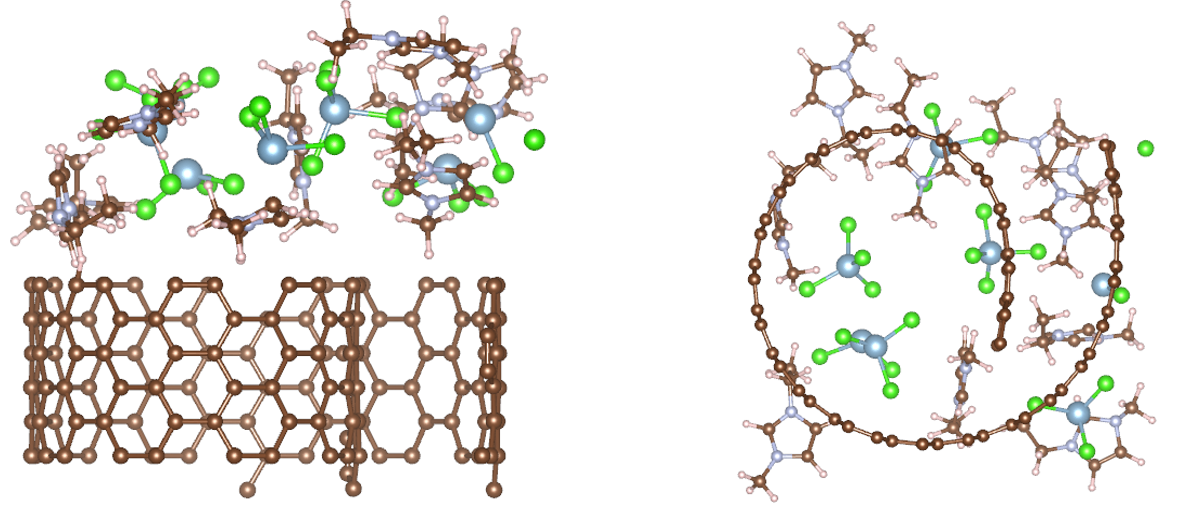
\includegraphics[width=0.48\textwidth]{fotos/interface side and top view.png}
\caption{Side and top views of the initial configuration of the interface between the carbon nanoscroll and the AlCl$_3$/[Emim]Cl electrolyte before the simulation.}
\label{fig:interface}
\end{figure}
There were also carried optimizations of the  \(AlCl_{3}^{-}\) molecule and the (Emim)Cl bound to a carbon atom on the edge of the nanoscroll. For this ones there where two diferent sites used. One where the molecules were bound to a carbon on top of the armchair, with a distance of 2 Å and others bound to a carbon of the bottom of the armchair with a distance of 3 Å. 
For the \(AlCl_{3}^{-}\) the molecule broke every time, regardless of the site it was originally, getting one Chlorine atom separated, but the atomic distance changed very little. For reference, the 4 Top sites of the \(AlCl_{3}^{-}\) are shown in the Figure~\ref{alcl3 sites} while the [Emim]Cl are shown in Figure~\ref{emil sites}
\begin{figure}[htbp]
\centering
%\includegraphics[width=0.35\textwidth]{fotos/alcl3 all sites.png}
\caption{Optimized \(AlCl_{3}^{-}\) molecule bound to the four different top sites in the nanoscroll}
\label{alcl3 sites}
\end{figure}

\begin{figure}[htbp]
\centering
%\includegraphics[width=0.35\textwidth]{fotos/emil sites.png}
\caption{Optimized [Emim]Cl molecule bound to the four different top sites in the nanoscroll}
\label{emil sites}
\end{figure}
For the Electrolyte, the only Chlorine there was, moved around, but the molecule remain stable, regardless of the type of bound. In this case the molecule moved closer to the nanoscroll more, compared to the previous \(AlCl_{3}^{-}\).\\
With these already optimized configurations, the adsorption energies of each one were calculated. This energy refers to the energy required to separate a system, whether composed of molecules, atoms, or electrons, and is calculated by subtracting from the energy of the system the energies of each of its parts separately; in this case, the total system energy minus that of the nanoscroll and that of the molecule.\cite{caldararu2017binding}

\begin{equation}E_{adsorption}=E_{system}-E_{scroll}-E_{molecule}\end{equation}
For the regular scroll an energy of -3539.71 Ry was obtained and for the one with vacuum -3528.71 Ry. For the optimized \(AlCl_{4}^{-}\) molecule the energy was -357.20 Ry, the \(AlCl_{4}^{-}\) of -277.89 Ry, and for the (Emim)Cl of 259,45 Ry. With these energies and those of each configuration, the graphics in Figure~\ref{3},~\ref{4} and~\ref{5} where generated. In Figure~\ref{3} we can see that in all three positions this energy is negative, and very close to each other, with a difference of 0.11 eV or less among all . These results imply that the molecules inside the nanoscroll are capable of detaching from it without the need to apply external energy, and the small variation of this energy among each position suggests that this can occur along the entire nanoscroll. This result is the most important of the investigation since it implies that nanoscrolls are capable of storing molecules in aluminum batteries, and that the process of extracting them from the cathode is optimal. On the other hand the Figures~\ref{4} and~\ref{5} show also negative energies, but this are way bigger than expected, and more so if compared with the ones for the \(AlCl_{4}^{-}\) molecule, this can be due to the fact that these molecules are placed at the edges of the nanoscroll, where the presence of dangling bonds and localized electronic states increases the reactivity and leads to stronger chemical interactions compared to the van der Waals-dominated intercalation sites.
\caption{Graph of the adsorption energies of the three different inside configurations of the \(AlCl_{4}^{-}\) molecule}
\begin{figure}[htbp]
\centering
%\includegraphics[width=0.35\textwidth]{fotos/AlCl4 Inside Sites.png}
\caption{Graph of the adsorption energies of the four different inside configurations of the \(AlCl_{4}^{-}\) molecule}
\label{3}
\end{figure}

\begin{figure}[htbp]
\centering
%\includegraphics[width=0.35\textwidth]{fotos/AlCl3 Sites.png}
\caption{Graph of the adsorption energies of the four different Up and Bottom configurations for the \(AlCl_{3}^{-}\) molecule}
\label{4}
\end{figure}

\begin{figure}[htbp]
\centering
%\includegraphics[width=0.35\textwidth]{fotos/Electrolyte Sites.png}
\caption{Graph of the adsorption energies of the four different Up configurations for the (Emim)Cl molecule}
\label{5}
\end{figure}


Another interesting result is generated by plotting the surfaces in terms of electron gain or loss, the total density of states of the system. This can be observed in Figure~\ref{6}, where the blue surfaces represent electron gain and the red ones electron loss. This implies that the \(AlCl_{4}^{-}\) molecules are subtracting electrons from the valence band of the scroll and storing them around the chlorine atoms.

To deeper understand this electronic interaction, we analyzed the Projected Density of States (PDOS), as shown in Figures~\ref{fig:pdos1} and~\ref{fig:pdos2}. In the pristine nanoscroll (Figure~\ref{fig:pdos1}, left), the states near the Fermi level are dominated by Carbon p-orbitals. Upon intercalation of AlCl$_4$ (Figure~\ref{fig:pdos1}, right, and Figure~\ref{fig:pdos2}), distinct molecular states (pink) appear in the valence band between -2.0 eV and -0.5 eV. The position of these states below the Fermi level confirms the charge transfer mechanism and the stability of the anion within the carbon host.

\begin{figure}[htbp]
\centering
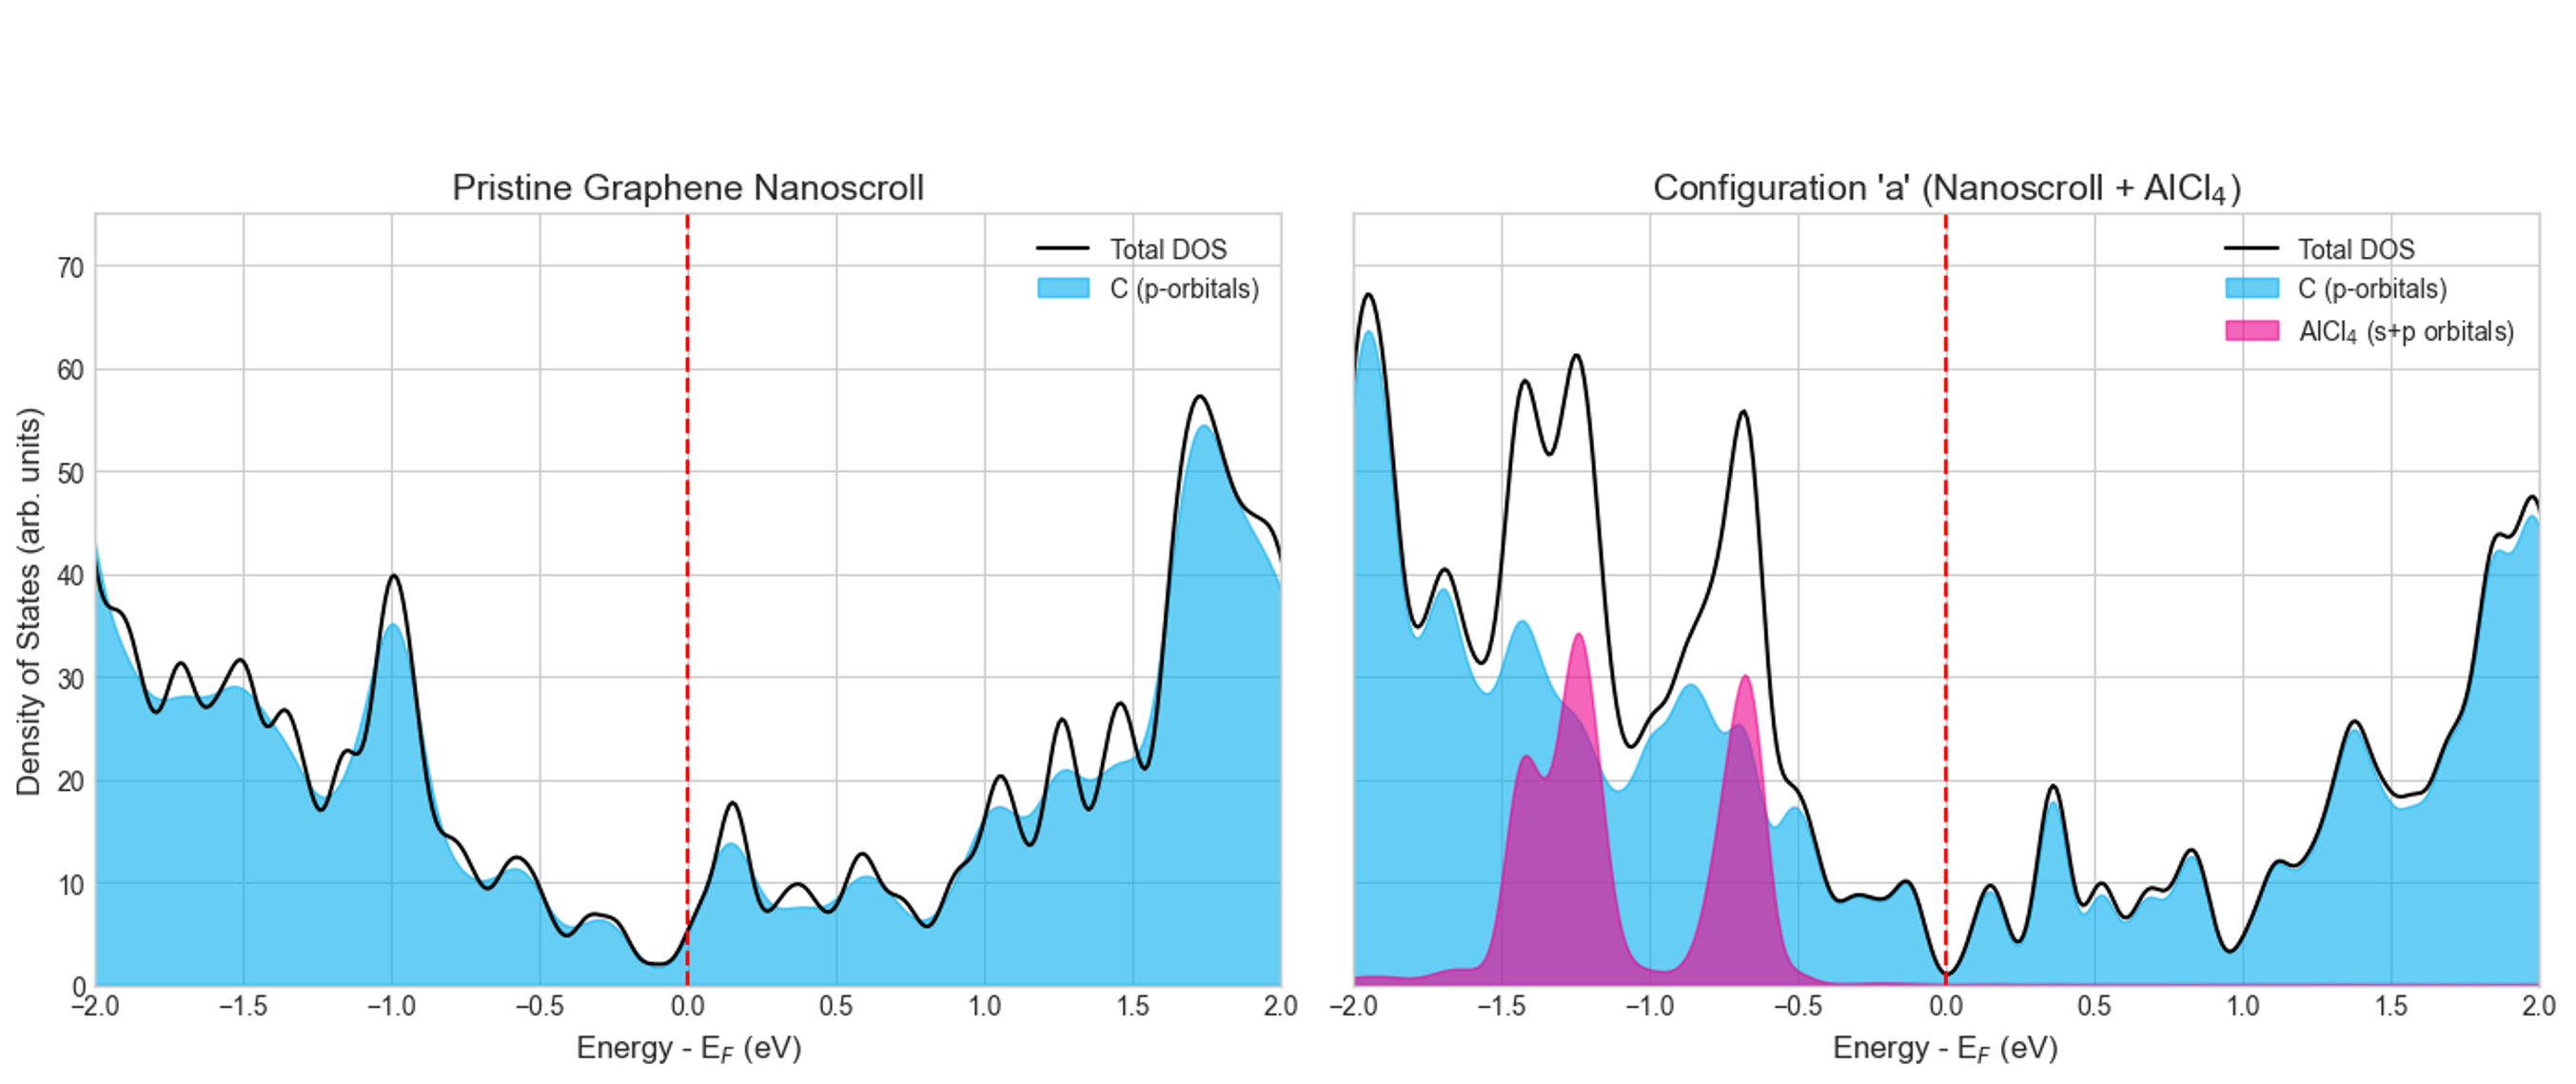
\includegraphics[width=0.48\textwidth]{fotos/PDOS pristine and config a.png}
\caption{Projected Density of States (PDOS) for the pristine graphene nanoscroll (left) and Configuration 'a' with intercalated AlCl$_4$ (right). The Carbon p-orbitals (blue) and AlCl$_4$ s+p orbitals (pink) are shown.}
\label{fig:pdos1}
\end{figure}

\begin{figure}[htbp]
\centering
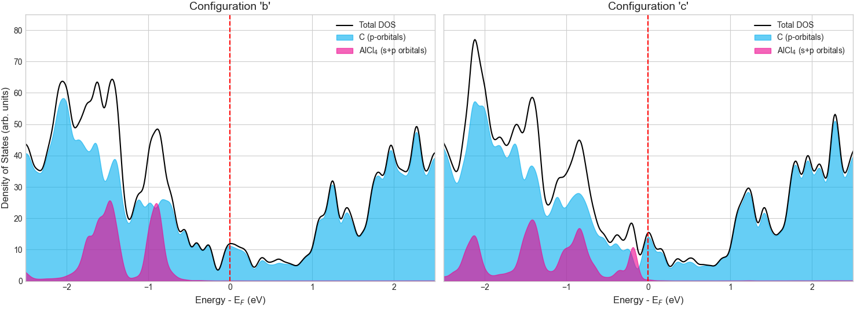
\includegraphics[width=0.48\textwidth]{fotos/PDOS config b and c.png}
\caption{PDOS for configurations 'b' and 'c', showing similar hybridization patterns of the AlCl$_4$ molecule within the nanoscroll.}
\label{fig:pdos2}
\end{figure} 

Finally, to characterize the structure of the solid electrolyte interphase (SEI) formed at the nanoscroll surface, we calculated the Radial Distribution Functions (RDFs) from the equilibrium trajectory. The results, presented in Figure~\ref{fig:rdf}, show the probability of finding specific electrolyte components at a distance $r$ from the carbon surface. The pronounced peaks at short distances indicate a strong ordering of the ionic liquid species at the interface. This layering suggests the formation of a stable SEI, where the specific orientation of [Emim]$^+$ and AlCl$_4^-$ ions facilitates the stability of the intercalation channels.

\begin{figure}[htbp]
\centering
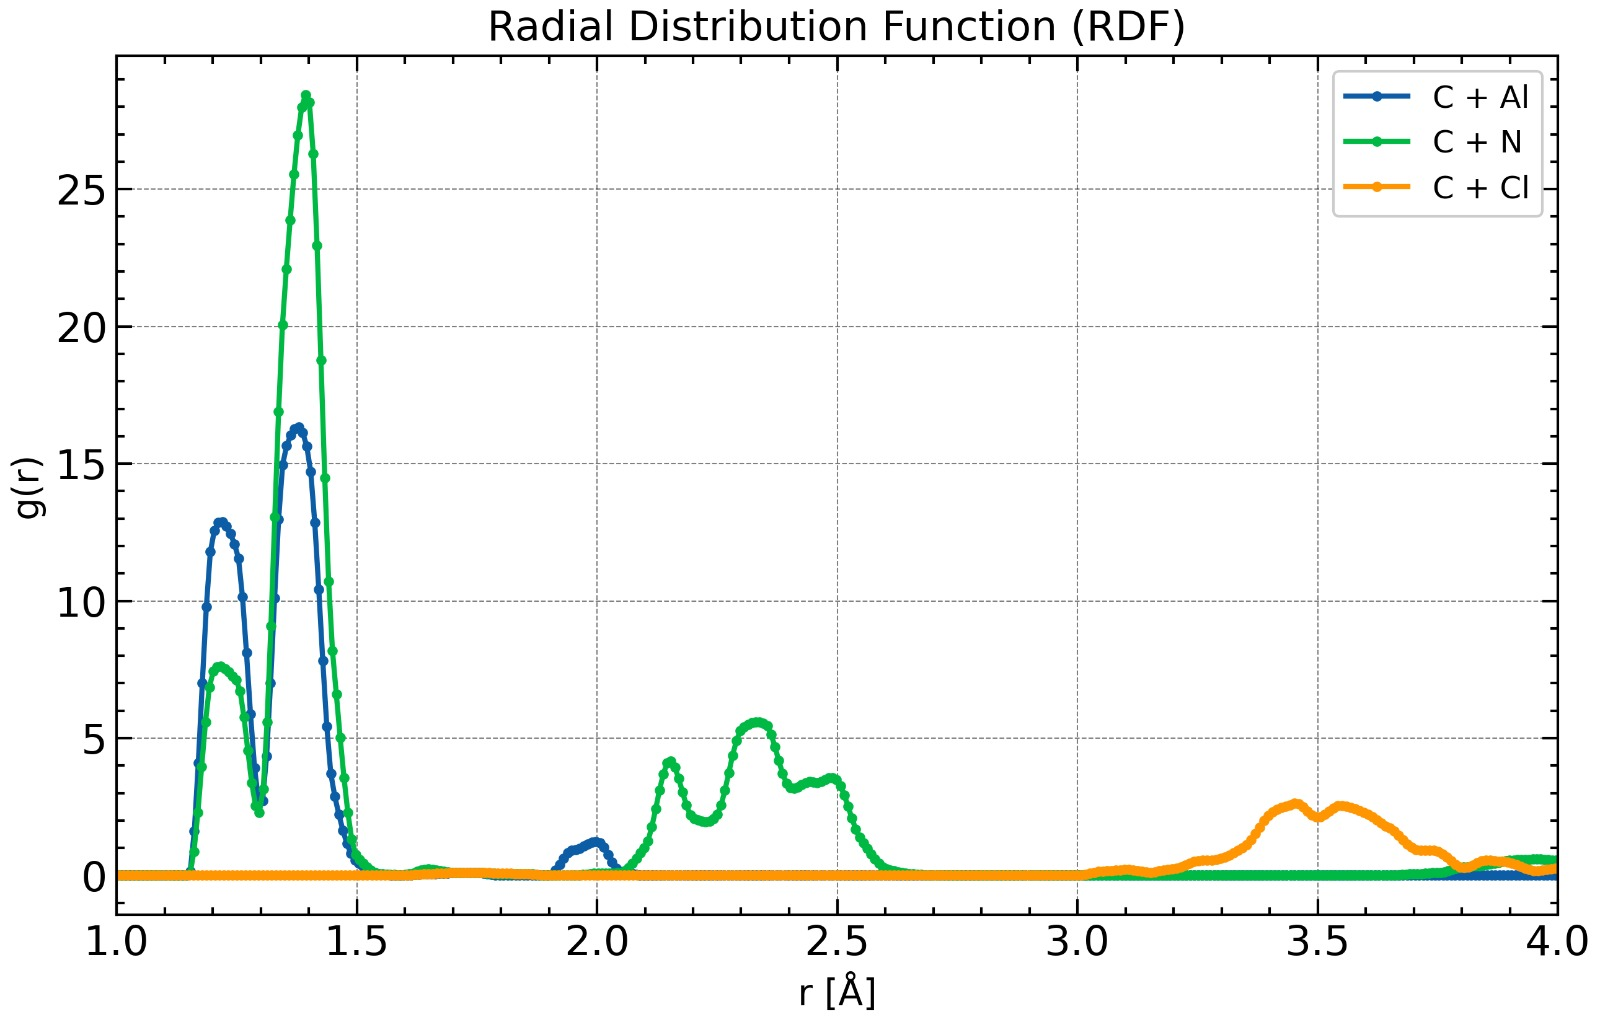
\includegraphics[width=0.48\textwidth]{fotos/RDF interface.jpeg}
\caption{Radial Distribution Functions (RDFs) of the electrolyte components relative to the carbon nanoscroll surface, depicting the structure of the SEI layer.}
\label{fig:rdf}
\end{figure} 
\begin{figure}[htbp]
\centering
% \includegraphics[width=0.35\textwidth]{fotos/Isosuperficies.png} % TODO: replace with valid image file
\fbox{\begin{minipage}{0.35\textwidth}\centering\vspace{3cm}[Isosuperficies figure --- replace Isosuperficies.png with a valid image]\vspace{3cm}\end{minipage}}
\caption{Isosurfaces of the four configurations. Blue regions represent electron gain, while red regions represent electron loss}
\label{6}
\end{figure}


Finally, with reference to Figure~\ref{7}, it shows the densities of states of each configuration and of the nanoscroll with respect to energy. The densities of states refer specifically to the electrons and to the existing states for each energy level\cite{di2010calculation}. It can be observed that the density is higher in the configurations than in the scroll below the Fermi energy. The latter refers to the highest energy level occupied by an electron at absolute zero.\cite{fan2025riemann}
\begin{figure}[htbp]
\centering
% \includegraphics[width=0.35\textwidth]{fotos/densidades de estados.png} % TODO: replace with valid image file
\fbox{\begin{minipage}{0.35\textwidth}\centering\vspace{3cm}[Densidades de estados figure --- replace densidades de estados.png with a valid image]\vspace{3cm}\end{minipage}}
\caption{Comparative graph of the densities of states of the configurations and of the nanoscroll as a function of energy}
\label{7}
\end{figure}
\newpage

\section{Conclusions}

This study provided a comprehensive computational analysis of Carbon Nanoscrolls as potential cathodes for Aluminum-ion batteries. Through a combination of DFT calculations and MD simulations, we successfully modeled the structural and electronic properties of the CNS-electrolyte interface.

The main conclusions are summarized as follows. First, the Archimedean spiral configuration of the CNS proved to be mechanically stable, accommodating the intercalation of large chloroaluminate anions without significant deformation. Regarding energetics, the AlCl$_4^-$ molecule exhibits a thermodynamically favorable adsorption within the scroll, strictly preferring a tetrahedral geometry over planar configurations.

Furthermore, PDOS analysis confirmed that the intercalation process is driven by charge transfer, with distinct AlCl$_4^-$ states appearing in the valence band, suggesting good electronic conductivity of the composite electrode. Finally, exploring the electrolyte interface revealed the formation of a stable SEI layer within 3.5 ps. Radial Distribution Functions highlighted a specific layering of [Emim]$^+$ and AlCl$_3$ species, which is critical for preventing electrode degradation and ensuring long-term cycle life.

These results validate the viability of Carbon Nanoscrolls as a robust and efficient cathode material, paving the way for further experimental validation and optimization of AIB technologies.

\section{Annex}
\begin{table}[h]
\begin{tabular}{|c|c|c|c|c|}
\hline
 & Site 1(eV) & Site 2(eV) & Site 3(eV) & Site 4(eV) \\
\hline
\(AlCl_{3}^{-}\) Top & -18.13094057 & -19.05818154 & -18.73649223 & -18.7860491
 \\
\hline
\(AlCl_{3}^{-}\) Bottom & -19.00617075  & -19.3908259
 & -18.86144769
 & -18.79487008
 \\
\hline
[Emim]Cl Top & -18.69416202 & -19.9466951 & -20.61650364 & -21.39861325 \\
\hline
[Emim]Cl Bottom & -22.59487735 & -20.31547336 & -20.01237038 & -20.17185944\\
\hline
\(AlCl_{4}\)& -0.21 & -0.1 & -0.12 & -0.13\\

\end{tabular}
\caption{Final Binding Energies of every simulated site}
\label{tab:ejemplo}
\end{table}
\bibliographystyle{unsrtnat}
\bibliography{library}



\end{document}